\documentclass[1p]{elsarticle_modified}
%\bibliographystyle{elsarticle-num}

%\usepackage[colorlinks]{hyperref}
%\usepackage{abbrmath_seonhwa} %\Abb, \Ascr, \Acal ,\Abf, \Afrak
\usepackage{amsfonts}
\usepackage{amssymb}
\usepackage{amsmath}
\usepackage{amsthm}
\usepackage{scalefnt}
\usepackage{amsbsy}
\usepackage{kotex}
\usepackage{caption}
\usepackage{subfig}
\usepackage{color}
\usepackage{graphicx}
\usepackage{xcolor} %% white, black, red, green, blue, cyan, magenta, yellow
\usepackage{float}
\usepackage{setspace}
\usepackage{hyperref}

\usepackage{tikz}
\usetikzlibrary{arrows}

\usepackage{multirow}
\usepackage{array} % fixed length table
\usepackage{hhline}

%%%%%%%%%%%%%%%%%%%%%
\makeatletter
\renewcommand*\env@matrix[1][\arraystretch]{%
	\edef\arraystretch{#1}%
	\hskip -\arraycolsep
	\let\@ifnextchar\new@ifnextchar
	\array{*\c@MaxMatrixCols c}}
\makeatother %https://tex.stackexchange.com/questions/14071/how-can-i-increase-the-line-spacing-in-a-matrix
%%%%%%%%%%%%%%%

\usepackage[normalem]{ulem}

\newcommand{\msout}[1]{\ifmmode\text{\sout{\ensuremath{#1}}}\else\sout{#1}\fi}
%SOURCE: \msout is \stkout macro in https://tex.stackexchange.com/questions/20609/strikeout-in-math-mode

\newcommand{\cancel}[1]{
	\ifmmode
	{\color{red}\msout{#1}}
	\else
	{\color{red}\sout{#1}}
	\fi
}

\newcommand{\add}[1]{
	{\color{blue}\uwave{#1}}
}

\newcommand{\replace}[2]{
	\ifmmode
	{\color{red}\msout{#1}}{\color{blue}\uwave{#2}}
	\else
	{\color{red}\sout{#1}}{\color{blue}\uwave{#2}}
	\fi
}

\newcommand{\Sol}{\mathcal{S}} %segment
\newcommand{\D}{D} %diagram
\newcommand{\A}{\mathcal{A}} %arc


%%%%%%%%%%%%%%%%%%%%%%%%%%%%%5 test

\def\sl{\operatorname{\textup{SL}}(2,\Cbb)}
\def\psl{\operatorname{\textup{PSL}}(2,\Cbb)}
\def\quan{\mkern 1mu \triangleright \mkern 1mu}

\theoremstyle{definition}
\newtheorem{thm}{Theorem}[section]
\newtheorem{prop}[thm]{Proposition}
\newtheorem{lem}[thm]{Lemma}
\newtheorem{ques}[thm]{Question}
\newtheorem{cor}[thm]{Corollary}
\newtheorem{defn}[thm]{Definition}
\newtheorem{exam}[thm]{Example}
\newtheorem{rmk}[thm]{Remark}
\newtheorem{alg}[thm]{Algorithm}

\newcommand{\I}{\sqrt{-1}}
\begin{document}

%\begin{frontmatter}
%
%\title{Boundary parabolic representations of knots up to 8 crossings}
%
%%% Group authors per affiliation:
%\author{Yunhi Cho} 
%\address{Department of Mathematics, University of Seoul, Seoul, Korea}
%\ead{yhcho@uos.ac.kr}
%
%
%\author{Seonhwa Kim} %\fnref{s_kim}}
%\address{Center for Geometry and Physics, Institute for Basic Science, Pohang, 37673, Korea}
%\ead{ryeona17@ibs.re.kr}
%
%\author{Hyuk Kim}
%\address{Department of Mathematical Sciences, Seoul National University, Seoul 08826, Korea}
%\ead{hyukkim@snu.ac.kr}
%
%\author{Seokbeom Yoon}
%\address{Department of Mathematical Sciences, Seoul National University, Seoul, 08826,  Korea}
%\ead{sbyoon15@snu.ac.kr}
%
%\begin{abstract}
%We find all boundary parabolic representation of knots up to 8 crossings.
%
%\end{abstract}
%\begin{keyword}
%    \MSC[2010] 57M25 
%\end{keyword}
%
%\end{frontmatter}

%\linenumbers
%\tableofcontents
%
\newcommand\colored[1]{\textcolor{white}{\rule[-0.35ex]{0.8em}{1.4ex}}\kern-0.8em\color{red} #1}%
%\newcommand\colored[1]{\textcolor{white}{ #1}\kern-2.17ex	\textcolor{white}{ #1}\kern-1.81ex	\textcolor{white}{ #1}\kern-2.15ex\color{red}#1	}

{\Large $\underline{12n_{0186}~(K12n_{0186})}$}

\setlength{\tabcolsep}{10pt}
\renewcommand{\arraystretch}{1.6}
\vspace{1cm}\begin{tabular}{m{100pt}>{\centering\arraybackslash}m{274pt}}
\multirow{5}{120pt}{
	\centering
	\includegraphics[width=112pt]{../../../GIT/diagram.site/Diagrams/png/2275_12n_0186.png}\\
\ \ \ A knot diagram\footnotemark}&
\allowdisplaybreaks
\textbf{Linearized knot diagam} \\
\cline{2-2}
 &
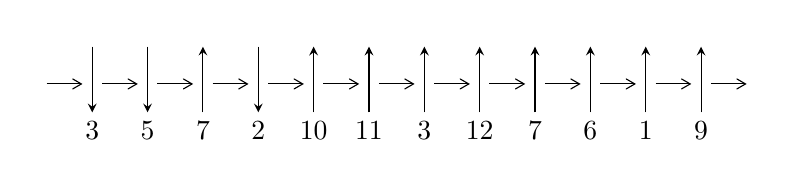
\begin{tikzpicture}[x=20pt, y=17pt]
	% nodes
	\node (C0) at (0, 0) {};
	\node (C1) at (1, 0) {};
	\node (C1U) at (1, +1) {};
	\node (C1D) at (1, -1) {3};

	\node (C2) at (2, 0) {};
	\node (C2U) at (2, +1) {};
	\node (C2D) at (2, -1) {5};

	\node (C3) at (3, 0) {};
	\node (C3U) at (3, +1) {};
	\node (C3D) at (3, -1) {7};

	\node (C4) at (4, 0) {};
	\node (C4U) at (4, +1) {};
	\node (C4D) at (4, -1) {2};

	\node (C5) at (5, 0) {};
	\node (C5U) at (5, +1) {};
	\node (C5D) at (5, -1) {10};

	\node (C6) at (6, 0) {};
	\node (C6U) at (6, +1) {};
	\node (C6D) at (6, -1) {11};

	\node (C7) at (7, 0) {};
	\node (C7U) at (7, +1) {};
	\node (C7D) at (7, -1) {3};

	\node (C8) at (8, 0) {};
	\node (C8U) at (8, +1) {};
	\node (C8D) at (8, -1) {12};

	\node (C9) at (9, 0) {};
	\node (C9U) at (9, +1) {};
	\node (C9D) at (9, -1) {7};

	\node (C10) at (10, 0) {};
	\node (C10U) at (10, +1) {};
	\node (C10D) at (10, -1) {6};

	\node (C11) at (11, 0) {};
	\node (C11U) at (11, +1) {};
	\node (C11D) at (11, -1) {1};

	\node (C12) at (12, 0) {};
	\node (C12U) at (12, +1) {};
	\node (C12D) at (12, -1) {9};
	\node (C13) at (13, 0) {};

	% arrows
	\draw[->,>={angle 60}]
	(C0) edge (C1) (C1) edge (C2) (C2) edge (C3) (C3) edge (C4) (C4) edge (C5) (C5) edge (C6) (C6) edge (C7) (C7) edge (C8) (C8) edge (C9) (C9) edge (C10) (C10) edge (C11) (C11) edge (C12) (C12) edge (C13) ;	\draw[->,>=stealth]
	(C1U) edge (C1D) (C2U) edge (C2D) (C3D) edge (C3U) (C4U) edge (C4D) (C5D) edge (C5U) (C6D) edge (C6U) (C7D) edge (C7U) (C8D) edge (C8U) (C9D) edge (C9U) (C10D) edge (C10U) (C11D) edge (C11U) (C12D) edge (C12U) ;
	\end{tikzpicture} \\
\hhline{~~} \\& 
\textbf{Solving Sequence} \\ \cline{2-2} 
 &
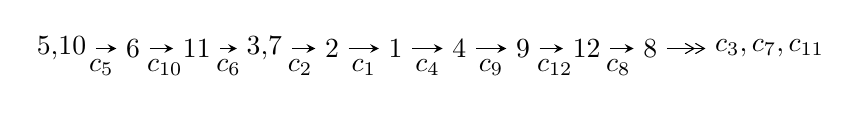
\begin{tikzpicture}[x=23pt, y=7pt]
	% node
	\node (A0) at (-1/8, 0) {5,10};
	\node (A1) at (1, 0) {6};
	\node (A2) at (2, 0) {11};
	\node (A3) at (49/16, 0) {3,7};
	\node (A4) at (33/8, 0) {2};
	\node (A5) at (41/8, 0) {1};
	\node (A6) at (49/8, 0) {4};
	\node (A7) at (57/8, 0) {9};
	\node (A8) at (65/8, 0) {12};
	\node (A9) at (73/8, 0) {8};
	\node (C1) at (1/2, -1) {$c_{5}$};
	\node (C2) at (3/2, -1) {$c_{10}$};
	\node (C3) at (5/2, -1) {$c_{6}$};
	\node (C4) at (29/8, -1) {$c_{2}$};
	\node (C5) at (37/8, -1) {$c_{1}$};
	\node (C6) at (45/8, -1) {$c_{4}$};
	\node (C7) at (53/8, -1) {$c_{9}$};
	\node (C8) at (61/8, -1) {$c_{12}$};
	\node (C9) at (69/8, -1) {$c_{8}$};
	\node (A10) at (11, 0) {$c_{3},c_{7},c_{11}$};

	% edge
	\draw[->,>=stealth]	
	(A0) edge (A1) (A1) edge (A2) (A2) edge (A3) (A3) edge (A4) (A4) edge (A5) (A5) edge (A6) (A6) edge (A7) (A7) edge (A8) (A8) edge (A9) ;
	\draw[->>,>={angle 60}]	
	(A9) edge (A10);
\end{tikzpicture} \\ 

\end{tabular} \\

\footnotetext{
The image of knot diagram is generated by the software ``\textbf{Draw programme}" developed by Andrew Bartholomew(\url{http://www.layer8.co.uk/maths/draw/index.htm\#Running-draw}), where we modified some parts for our purpose(\url{https://github.com/CATsTAILs/LinksPainter}).
}\phantom \\ \newline 
\centering \textbf{Ideals for irreducible components\footnotemark of $X_{\text{par}}$} 
 
\begin{align*}
I^u_{1}&=\langle 
3.22078\times10^{25} u^{51}-8.93113\times10^{25} u^{50}+\cdots+5.70770\times10^{25} b+5.96223\times10^{25},\\
\phantom{I^u_{1}}&\phantom{= \langle  }5.22434\times10^{25} u^{51}-2.15422\times10^{25} u^{50}+\cdots+5.70770\times10^{25} a-1.21095\times10^{26},\;u^{52}-2 u^{51}+\cdots- u^2+1\rangle \\
I^u_{2}&=\langle 
b+1,\;2 u^7- u^6-5 u^5+2 u^4+3 u^3+a+2 u-1,\;u^8- u^7-3 u^6+2 u^5+3 u^4-2 u-1\rangle \\
\\
\end{align*}
\raggedright * 2 irreducible components of $\dim_{\mathbb{C}}=0$, with total 60 representations.\\
\footnotetext{All coefficients of polynomials are rational numbers. But the coefficients are sometimes approximated in decimal forms when there is not enough margin.}
\newpage
\renewcommand{\arraystretch}{1}
\centering \section*{I. $I^u_{1}= \langle 3.22\times10^{25} u^{51}-8.93\times10^{25} u^{50}+\cdots+5.71\times10^{25} b+5.96\times10^{25},\;5.22\times10^{25} u^{51}-2.15\times10^{25} u^{50}+\cdots+5.71\times10^{25} a-1.21\times10^{26},\;u^{52}-2 u^{51}+\cdots- u^2+1 \rangle$}
\flushleft \textbf{(i) Arc colorings}\\
\begin{tabular}{m{7pt} m{180pt} m{7pt} m{180pt} }
\flushright $a_{5}=$&$\begin{pmatrix}1\\0\end{pmatrix}$ \\
\flushright $a_{10}=$&$\begin{pmatrix}0\\u\end{pmatrix}$ \\
\flushright $a_{6}=$&$\begin{pmatrix}1\\- u^2\end{pmatrix}$ \\
\flushright $a_{11}=$&$\begin{pmatrix}u\\- u^3+u\end{pmatrix}$ \\
\flushright $a_{3}=$&$\begin{pmatrix}-0.915316 u^{51}+0.377424 u^{50}+\cdots-0.305015 u+2.12160\\-0.564287 u^{51}+1.56475 u^{50}+\cdots+0.657034 u-1.04459\end{pmatrix}$ \\
\flushright $a_{7}=$&$\begin{pmatrix}- u^2+1\\u^4-2 u^2\end{pmatrix}$ \\
\flushright $a_{2}=$&$\begin{pmatrix}-1.47960 u^{51}+1.94218 u^{50}+\cdots+0.352020 u+1.07701\\-0.564287 u^{51}+1.56475 u^{50}+\cdots+0.657034 u-1.04459\end{pmatrix}$ \\
\flushright $a_{1}=$&$\begin{pmatrix}-1.18721 u^{51}+3.15641 u^{50}+\cdots+2.25837 u-0.599223\\0.268382 u^{51}-0.928704 u^{50}+\cdots-0.481556 u+0.106979\end{pmatrix}$ \\
\flushright $a_{4}=$&$\begin{pmatrix}-1.04390 u^{51}+0.780635 u^{50}+\cdots-0.415024 u+1.93894\\-0.616840 u^{51}+1.83391 u^{50}+\cdots+0.779891 u-1.08938\end{pmatrix}$ \\
\flushright $a_{9}=$&$\begin{pmatrix}- u^5+2 u^3- u\\u^7-3 u^5+2 u^3+u\end{pmatrix}$ \\
\flushright $a_{12}=$&$\begin{pmatrix}-0.594106 u^{51}+1.79472 u^{50}+\cdots+1.62921 u-0.588090\\-0.276947 u^{51}+0.473102 u^{50}+\cdots+0.517256 u+0.0584887\end{pmatrix}$ \\
\flushright $a_{8}=$&$\begin{pmatrix}0.285029 u^{51}-0.390403 u^{50}+\cdots-1.33955 u+0.209160\\-0.492416 u^{51}+1.54733 u^{50}+\cdots+0.722296 u-0.103429\end{pmatrix}$\\&\end{tabular}
\flushleft \textbf{(ii) Obstruction class $= -1$}\\~\\
\flushleft \textbf{(iii) Cusp Shapes $= \frac{1240657506593977463220736159}{57076965857356338641202335} u^{51}-\frac{507731546315019686665244629}{57076965857356338641202335} u^{50}+\cdots-\frac{1047474987399803989773483394}{57076965857356338641202335} u-\frac{421248860824180893040358514}{57076965857356338641202335}$}\\~\\
\newpage\renewcommand{\arraystretch}{1}
\flushleft \textbf{(iv) u-Polynomials at the component}\newline \\
\begin{tabular}{m{50pt}|m{274pt}}
Crossings & \hspace{64pt}u-Polynomials at each crossing \\
\hline $$\begin{aligned}c_{1}\end{aligned}$$&$\begin{aligned}
&u^{52}+15 u^{51}+\cdots+154 u+1
\end{aligned}$\\
\hline $$\begin{aligned}c_{2},c_{4}\end{aligned}$$&$\begin{aligned}
&u^{52}-9 u^{51}+\cdots-18 u+1
\end{aligned}$\\
\hline $$\begin{aligned}c_{3},c_{7}\end{aligned}$$&$\begin{aligned}
&u^{52}-3 u^{51}+\cdots-4480 u+256
\end{aligned}$\\
\hline $$\begin{aligned}c_{5},c_{6},c_{10}\end{aligned}$$&$\begin{aligned}
&u^{52}-2 u^{51}+\cdots- u^2+1
\end{aligned}$\\
\hline $$\begin{aligned}c_{8},c_{12}\end{aligned}$$&$\begin{aligned}
&u^{52}-2 u^{51}+\cdots-4 u+1
\end{aligned}$\\
\hline $$\begin{aligned}c_{9}\end{aligned}$$&$\begin{aligned}
&u^{52}+6 u^{51}+\cdots+880 u+4025
\end{aligned}$\\
\hline $$\begin{aligned}c_{11}\end{aligned}$$&$\begin{aligned}
&u^{52}-30 u^{51}+\cdots-2 u+1
\end{aligned}$\\
\hline
\end{tabular}\\~\\
\newpage\renewcommand{\arraystretch}{1}
\flushleft \textbf{(v) Riley Polynomials at the component}\newline \\
\begin{tabular}{m{50pt}|m{274pt}}
Crossings & \hspace{64pt}Riley Polynomials at each crossing \\
\hline $$\begin{aligned}c_{1}\end{aligned}$$&$\begin{aligned}
&y^{52}+53 y^{51}+\cdots-8978 y+1
\end{aligned}$\\
\hline $$\begin{aligned}c_{2},c_{4}\end{aligned}$$&$\begin{aligned}
&y^{52}-15 y^{51}+\cdots-154 y+1
\end{aligned}$\\
\hline $$\begin{aligned}c_{3},c_{7}\end{aligned}$$&$\begin{aligned}
&y^{52}-51 y^{51}+\cdots-6209536 y+65536
\end{aligned}$\\
\hline $$\begin{aligned}c_{5},c_{6},c_{10}\end{aligned}$$&$\begin{aligned}
&y^{52}-50 y^{51}+\cdots-2 y+1
\end{aligned}$\\
\hline $$\begin{aligned}c_{8},c_{12}\end{aligned}$$&$\begin{aligned}
&y^{52}-30 y^{51}+\cdots-2 y+1
\end{aligned}$\\
\hline $$\begin{aligned}c_{9}\end{aligned}$$&$\begin{aligned}
&y^{52}-26 y^{51}+\cdots-386280850 y+16200625
\end{aligned}$\\
\hline $$\begin{aligned}c_{11}\end{aligned}$$&$\begin{aligned}
&y^{52}-14 y^{51}+\cdots-22 y+1
\end{aligned}$\\
\hline
\end{tabular}\\~\\
\newpage\flushleft \textbf{(vi) Complex Volumes and Cusp Shapes}
$$\begin{array}{c|c|c}  
\text{Solutions to }I^u_{1}& \I (\text{vol} + \sqrt{-1}CS) & \text{Cusp shape}\\
 \hline 
\begin{aligned}
u &= -0.596040 + 0.685350 I \\
a &= -0.303738 - 0.109363 I \\
b &= \phantom{-}1.035020 - 0.836655 I\end{aligned}
 & \phantom{-}6.06449 + 5.90411 I & \phantom{-}8.42870 - 2.86873 I \\ \hline\begin{aligned}
u &= -0.596040 - 0.685350 I \\
a &= -0.303738 + 0.109363 I \\
b &= \phantom{-}1.035020 + 0.836655 I\end{aligned}
 & \phantom{-}6.06449 - 5.90411 I & \phantom{-}8.42870 + 2.86873 I \\ \hline\begin{aligned}
u &= -0.461943 + 0.763402 I \\
a &= \phantom{-}0.92002 - 1.14323 I \\
b &= \phantom{-}1.15749 + 0.84016 I\end{aligned}
 & \phantom{-}5.61921 - 10.76330 I & \phantom{-}7.42388 + 7.81134 I \\ \hline\begin{aligned}
u &= -0.461943 - 0.763402 I \\
a &= \phantom{-}0.92002 + 1.14323 I \\
b &= \phantom{-}1.15749 - 0.84016 I\end{aligned}
 & \phantom{-}5.61921 + 10.76330 I & \phantom{-}7.42388 - 7.81134 I \\ \hline\begin{aligned}
u &= \phantom{-}0.600467 + 0.630929 I \\
a &= -0.194035 - 0.006330 I \\
b &= \phantom{-}0.804140 + 0.798246 I\end{aligned}
 & \phantom{-}2.75283 - 0.63628 I & \phantom{-}6.47155 - 0.50182 I \\ \hline\begin{aligned}
u &= \phantom{-}0.600467 - 0.630929 I \\
a &= -0.194035 + 0.006330 I \\
b &= \phantom{-}0.804140 - 0.798246 I\end{aligned}
 & \phantom{-}2.75283 + 0.63628 I & \phantom{-}6.47155 + 0.50182 I \\ \hline\begin{aligned}
u &= \phantom{-}0.429595 + 0.756706 I \\
a &= \phantom{-}1.011620 + 0.980800 I \\
b &= \phantom{-}1.000840 - 0.771858 I\end{aligned}
 & \phantom{-}2.14152 + 5.31582 I & \phantom{-}4.93660 - 5.12952 I \\ \hline\begin{aligned}
u &= \phantom{-}0.429595 - 0.756706 I \\
a &= \phantom{-}1.011620 - 0.980800 I \\
b &= \phantom{-}1.000840 + 0.771858 I\end{aligned}
 & \phantom{-}2.14152 - 5.31582 I & \phantom{-}4.93660 + 5.12952 I \\ \hline\begin{aligned}
u &= -0.428853 + 0.704754 I \\
a &= \phantom{-}1.28272 - 0.99964 I \\
b &= \phantom{-}0.810880 + 0.929645 I\end{aligned}
 & \phantom{-}6.77557 - 0.63032 I & \phantom{-}9.03919 + 2.39060 I \\ \hline\begin{aligned}
u &= -0.428853 - 0.704754 I \\
a &= \phantom{-}1.28272 + 0.99964 I \\
b &= \phantom{-}0.810880 - 0.929645 I\end{aligned}
 & \phantom{-}6.77557 + 0.63032 I & \phantom{-}9.03919 - 2.39060 I\\
 \hline 
 \end{array}$$\newpage$$\begin{array}{c|c|c}  
\text{Solutions to }I^u_{1}& \I (\text{vol} + \sqrt{-1}CS) & \text{Cusp shape}\\
 \hline 
\begin{aligned}
u &= -0.529637 + 0.629472 I \\
a &= -0.312532 + 0.180815 I \\
b &= \phantom{-}0.675424 - 1.090410 I\end{aligned}
 & \phantom{-}7.14701 - 3.78883 I & \phantom{-}9.80206 + 4.18447 I \\ \hline\begin{aligned}
u &= -0.529637 - 0.629472 I \\
a &= -0.312532 - 0.180815 I \\
b &= \phantom{-}0.675424 + 1.090410 I\end{aligned}
 & \phantom{-}7.14701 + 3.78883 I & \phantom{-}9.80206 - 4.18447 I \\ \hline\begin{aligned}
u &= \phantom{-}0.089818 + 0.804779 I \\
a &= \phantom{-}0.976159 + 0.124090 I \\
b &= \phantom{-}0.652722 - 0.112944 I\end{aligned}
 & -3.05621 + 2.81915 I & \phantom{-}8.84773 - 4.69108 I \\ \hline\begin{aligned}
u &= \phantom{-}0.089818 - 0.804779 I \\
a &= \phantom{-}0.976159 - 0.124090 I \\
b &= \phantom{-}0.652722 + 0.112944 I\end{aligned}
 & -3.05621 - 2.81915 I & \phantom{-}8.84773 + 4.69108 I \\ \hline\begin{aligned}
u &= \phantom{-}1.160150 + 0.341361 I \\
a &= \phantom{-}0.444553 + 0.408247 I \\
b &= \phantom{-}0.621048 - 0.094499 I\end{aligned}
 & \phantom{-}0.200968 + 1.333880 I & \phantom{-0.000000 } 0 \\ \hline\begin{aligned}
u &= \phantom{-}1.160150 - 0.341361 I \\
a &= \phantom{-}0.444553 - 0.408247 I \\
b &= \phantom{-}0.621048 + 0.094499 I\end{aligned}
 & \phantom{-}0.200968 - 1.333880 I & \phantom{-0.000000 } 0 \\ \hline\begin{aligned}
u &= -1.305710 + 0.022937 I \\
a &= \phantom{-}0.482228 + 0.442327 I \\
b &= -1.42955 - 0.12934 I\end{aligned}
 & \phantom{-}1.369850 - 0.105601 I & \phantom{-0.000000 } 0 \\ \hline\begin{aligned}
u &= -1.305710 - 0.022937 I \\
a &= \phantom{-}0.482228 - 0.442327 I \\
b &= -1.42955 + 0.12934 I\end{aligned}
 & \phantom{-}1.369850 + 0.105601 I & \phantom{-0.000000 } 0 \\ \hline\begin{aligned}
u &= -1.31861\phantom{ +0.000000I} \\
a &= \phantom{-}1.09514\phantom{ +0.000000I} \\
b &= \phantom{-}0.151920\phantom{ +0.000000I}\end{aligned}
 & \phantom{-}6.40470\phantom{ +0.000000I} & \phantom{-0.000000 } 0 \\ \hline\begin{aligned}
u &= \phantom{-}1.317970 + 0.092549 I \\
a &= \phantom{-}0.81132 - 1.44084 I \\
b &= -1.34968 + 0.57134 I\end{aligned}
 & \phantom{-}2.18752 + 3.25685 I & \phantom{-0.000000 } 0\\
 \hline 
 \end{array}$$\newpage$$\begin{array}{c|c|c}  
\text{Solutions to }I^u_{1}& \I (\text{vol} + \sqrt{-1}CS) & \text{Cusp shape}\\
 \hline 
\begin{aligned}
u &= \phantom{-}1.317970 - 0.092549 I \\
a &= \phantom{-}0.81132 + 1.44084 I \\
b &= -1.34968 - 0.57134 I\end{aligned}
 & \phantom{-}2.18752 - 3.25685 I & \phantom{-0.000000 } 0 \\ \hline\begin{aligned}
u &= -1.311760 + 0.358837 I \\
a &= \phantom{-}0.394809 - 0.696031 I \\
b &= \phantom{-}0.728756 + 0.259803 I\end{aligned}
 & \phantom{-}1.32923 - 7.01296 I & \phantom{-0.000000 } 0 \\ \hline\begin{aligned}
u &= -1.311760 - 0.358837 I \\
a &= \phantom{-}0.394809 + 0.696031 I \\
b &= \phantom{-}0.728756 - 0.259803 I\end{aligned}
 & \phantom{-}1.32923 + 7.01296 I & \phantom{-0.000000 } 0 \\ \hline\begin{aligned}
u &= \phantom{-}1.390960 + 0.114127 I \\
a &= \phantom{-}0.57698 - 1.72339 I \\
b &= -0.723456 + 0.697653 I\end{aligned}
 & \phantom{-}3.42681 + 2.63296 I & \phantom{-0.000000 } 0 \\ \hline\begin{aligned}
u &= \phantom{-}1.390960 - 0.114127 I \\
a &= \phantom{-}0.57698 + 1.72339 I \\
b &= -0.723456 - 0.697653 I\end{aligned}
 & \phantom{-}3.42681 - 2.63296 I & \phantom{-0.000000 } 0 \\ \hline\begin{aligned}
u &= \phantom{-}1.40302\phantom{ +0.000000I} \\
a &= -13.7171\phantom{ +0.000000I} \\
b &= -1.00767\phantom{ +0.000000I}\end{aligned}
 & \phantom{-}4.91335\phantom{ +0.000000I} & \phantom{-0.000000 } 0 \\ \hline\begin{aligned}
u &= -1.404190 + 0.159019 I \\
a &= \phantom{-}0.27827 + 1.88427 I \\
b &= -0.535802 - 1.135950 I\end{aligned}
 & \phantom{-}5.89367 - 6.10396 I & \phantom{-0.000000 } 0 \\ \hline\begin{aligned}
u &= -1.404190 - 0.159019 I \\
a &= \phantom{-}0.27827 - 1.88427 I \\
b &= -0.535802 + 1.135950 I\end{aligned}
 & \phantom{-}5.89367 + 6.10396 I & \phantom{-0.000000 } 0 \\ \hline\begin{aligned}
u &= \phantom{-}0.289349 + 0.491612 I \\
a &= -0.104933 - 0.935937 I \\
b &= -0.665776 + 0.817316 I\end{aligned}
 & \phantom{-}0.49136 + 3.75076 I & \phantom{-}5.76906 - 8.97851 I \\ \hline\begin{aligned}
u &= \phantom{-}0.289349 - 0.491612 I \\
a &= -0.104933 + 0.935937 I \\
b &= -0.665776 - 0.817316 I\end{aligned}
 & \phantom{-}0.49136 - 3.75076 I & \phantom{-}5.76906 + 8.97851 I\\
 \hline 
 \end{array}$$\newpage$$\begin{array}{c|c|c}  
\text{Solutions to }I^u_{1}& \I (\text{vol} + \sqrt{-1}CS) & \text{Cusp shape}\\
 \hline 
\begin{aligned}
u &= -1.43138 + 0.07294 I \\
a &= \phantom{-}1.036390 + 0.944754 I \\
b &= -0.270270 - 0.184770 I\end{aligned}
 & \phantom{-}6.54809 - 0.25945 I & \phantom{-0.000000 } 0 \\ \hline\begin{aligned}
u &= -1.43138 - 0.07294 I \\
a &= \phantom{-}1.036390 - 0.944754 I \\
b &= -0.270270 + 0.184770 I\end{aligned}
 & \phantom{-}6.54809 + 0.25945 I & \phantom{-0.000000 } 0 \\ \hline\begin{aligned}
u &= \phantom{-}1.47938 + 0.26376 I \\
a &= \phantom{-}0.37431 + 1.88780 I \\
b &= \phantom{-}0.977064 - 0.921748 I\end{aligned}
 & \phantom{-}12.93400 + 4.17895 I & \phantom{-0.000000 } 0 \\ \hline\begin{aligned}
u &= \phantom{-}1.47938 - 0.26376 I \\
a &= \phantom{-}0.37431 - 1.88780 I \\
b &= \phantom{-}0.977064 + 0.921748 I\end{aligned}
 & \phantom{-}12.93400 - 4.17895 I & \phantom{-0.000000 } 0 \\ \hline\begin{aligned}
u &= \phantom{-}0.355651 + 0.332212 I \\
a &= \phantom{-}2.25163 - 0.94682 I \\
b &= -0.586013 - 0.340416 I\end{aligned}
 & \phantom{-}0.96467 - 1.11364 I & \phantom{-}8.10661 - 2.28473 I \\ \hline\begin{aligned}
u &= \phantom{-}0.355651 - 0.332212 I \\
a &= \phantom{-}2.25163 + 0.94682 I \\
b &= -0.586013 + 0.340416 I\end{aligned}
 & \phantom{-}0.96467 + 1.11364 I & \phantom{-}8.10661 + 2.28473 I \\ \hline\begin{aligned}
u &= -1.48991 + 0.28027 I \\
a &= \phantom{-}0.08758 - 1.83114 I \\
b &= \phantom{-}1.125690 + 0.835388 I\end{aligned}
 & \phantom{-}8.35025 - 9.10360 I & \phantom{-0.000000 } 0 \\ \hline\begin{aligned}
u &= -1.48991 - 0.28027 I \\
a &= \phantom{-}0.08758 + 1.83114 I \\
b &= \phantom{-}1.125690 - 0.835388 I\end{aligned}
 & \phantom{-}8.35025 + 9.10360 I & \phantom{-0.000000 } 0 \\ \hline\begin{aligned}
u &= \phantom{-}1.50299 + 0.21204 I \\
a &= -1.01775 - 1.30127 I \\
b &= \phantom{-}0.71828 + 1.28058 I\end{aligned}
 & \phantom{-}13.7566 + 6.8511 I & \phantom{-0.000000 } 0 \\ \hline\begin{aligned}
u &= \phantom{-}1.50299 - 0.21204 I \\
a &= -1.01775 + 1.30127 I \\
b &= \phantom{-}0.71828 - 1.28058 I\end{aligned}
 & \phantom{-}13.7566 - 6.8511 I & \phantom{-0.000000 } 0\\
 \hline 
 \end{array}$$\newpage$$\begin{array}{c|c|c}  
\text{Solutions to }I^u_{1}& \I (\text{vol} + \sqrt{-1}CS) & \text{Cusp shape}\\
 \hline 
\begin{aligned}
u &= \phantom{-}1.50262 + 0.27770 I \\
a &= -0.05829 + 1.98831 I \\
b &= \phantom{-}1.23801 - 0.89513 I\end{aligned}
 & \phantom{-}11.9860 + 14.5665 I & \phantom{-0.000000 } 0 \\ \hline\begin{aligned}
u &= \phantom{-}1.50262 - 0.27770 I \\
a &= -0.05829 - 1.98831 I \\
b &= \phantom{-}1.23801 + 0.89513 I\end{aligned}
 & \phantom{-}11.9860 - 14.5665 I & \phantom{-0.000000 } 0 \\ \hline\begin{aligned}
u &= -1.51858 + 0.19470 I \\
a &= -0.846488 + 1.031250 I \\
b &= \phantom{-}0.703551 - 1.024970 I\end{aligned}
 & \phantom{-}9.67287 - 2.30932 I & \phantom{-0.000000 } 0 \\ \hline\begin{aligned}
u &= -1.51858 - 0.19470 I \\
a &= -0.846488 - 1.031250 I \\
b &= \phantom{-}0.703551 + 1.024970 I\end{aligned}
 & \phantom{-}9.67287 + 2.30932 I & \phantom{-0.000000 } 0 \\ \hline\begin{aligned}
u &= -0.076509 + 0.456871 I \\
a &= -1.054590 + 0.666345 I \\
b &= -1.310420 - 0.236305 I\end{aligned}
 & -2.05132 - 1.32678 I & -0.14980 + 4.04076 I \\ \hline\begin{aligned}
u &= -0.076509 - 0.456871 I \\
a &= -1.054590 - 0.666345 I \\
b &= -1.310420 + 0.236305 I\end{aligned}
 & -2.05132 + 1.32678 I & -0.14980 - 4.04076 I \\ \hline\begin{aligned}
u &= \phantom{-}0.452272\phantom{ +0.000000I} \\
a &= \phantom{-}0.656563\phantom{ +0.000000I} \\
b &= \phantom{-}0.108480\phantom{ +0.000000I}\end{aligned}
 & \phantom{-}0.718769\phantom{ +0.000000I} & \phantom{-}13.9480\phantom{ +0.000000I} \\ \hline\begin{aligned}
u &= \phantom{-}1.53851 + 0.20821 I \\
a &= -1.040950 - 0.804099 I \\
b &= \phantom{-}0.925560 + 0.944868 I\end{aligned}
 & \phantom{-}13.09740 - 2.67801 I & \phantom{-0.000000 } 0 \\ \hline\begin{aligned}
u &= \phantom{-}1.53851 - 0.20821 I \\
a &= -1.040950 + 0.804099 I \\
b &= \phantom{-}0.925560 - 0.944868 I\end{aligned}
 & \phantom{-}13.09740 + 2.67801 I & \phantom{-0.000000 } 0 \\ \hline\begin{aligned}
u &= -0.202886 + 0.379947 I \\
a &= -0.30999 + 1.78499 I \\
b &= -0.885931 - 0.291667 I\end{aligned}
 & -1.66844 - 0.85066 I & -1.89079 + 2.59214 I\\
 \hline 
 \end{array}$$\newpage$$\begin{array}{c|c|c}  
\text{Solutions to }I^u_{1}& \I (\text{vol} + \sqrt{-1}CS) & \text{Cusp shape}\\
 \hline 
\begin{aligned}
u &= -0.202886 - 0.379947 I \\
a &= -0.30999 - 1.78499 I \\
b &= -0.885931 + 0.291667 I\end{aligned}
 & -1.66844 + 0.85066 I & -1.89079 - 2.59214 I \\ \hline\begin{aligned}
u &= -0.336802\phantom{ +0.000000I} \\
a &= \phantom{-}6.59478\phantom{ +0.000000I} \\
b &= -1.08789\phantom{ +0.000000I}\end{aligned}
 & -0.454350\phantom{ +0.000000I} & \phantom{-}34.0590\phantom{ +0.000000I}\\
 \hline 
 \end{array}$$\newpage\newpage\renewcommand{\arraystretch}{1}
\centering \section*{II. $I^u_{2}= \langle b+1,\;2 u^7- u^6-5 u^5+2 u^4+3 u^3+a+2 u-1,\;u^8- u^7-3 u^6+2 u^5+3 u^4-2 u-1 \rangle$}
\flushleft \textbf{(i) Arc colorings}\\
\begin{tabular}{m{7pt} m{180pt} m{7pt} m{180pt} }
\flushright $a_{5}=$&$\begin{pmatrix}1\\0\end{pmatrix}$ \\
\flushright $a_{10}=$&$\begin{pmatrix}0\\u\end{pmatrix}$ \\
\flushright $a_{6}=$&$\begin{pmatrix}1\\- u^2\end{pmatrix}$ \\
\flushright $a_{11}=$&$\begin{pmatrix}u\\- u^3+u\end{pmatrix}$ \\
\flushright $a_{3}=$&$\begin{pmatrix}-2 u^7+u^6+5 u^5-2 u^4-3 u^3-2 u+1\\-1\end{pmatrix}$ \\
\flushright $a_{7}=$&$\begin{pmatrix}- u^2+1\\u^4-2 u^2\end{pmatrix}$ \\
\flushright $a_{2}=$&$\begin{pmatrix}-2 u^7+u^6+5 u^5-2 u^4-3 u^3-2 u\\-1\end{pmatrix}$ \\
\flushright $a_{1}=$&$\begin{pmatrix}-1\\0\end{pmatrix}$ \\
\flushright $a_{4}=$&$\begin{pmatrix}-2 u^7+u^6+5 u^5-2 u^4-3 u^3-2 u+1\\-1\end{pmatrix}$ \\
\flushright $a_{9}=$&$\begin{pmatrix}- u^5+2 u^3- u\\u^7-3 u^5+2 u^3+u\end{pmatrix}$ \\
\flushright $a_{12}=$&$\begin{pmatrix}- u^3+2 u\\- u^3+u\end{pmatrix}$ \\
\flushright $a_{8}=$&$\begin{pmatrix}- u^2+1\\u^4-2 u^2\end{pmatrix}$\\&\end{tabular}
\flushleft \textbf{(ii) Obstruction class $= 1$}\\~\\
\flushleft \textbf{(iii) Cusp Shapes $= -4 u^7- u^6+10 u^5+3 u^4-6 u^3-2 u^2-4 u-1$}\\~\\
\newpage\renewcommand{\arraystretch}{1}
\flushleft \textbf{(iv) u-Polynomials at the component}\newline \\
\begin{tabular}{m{50pt}|m{274pt}}
Crossings & \hspace{64pt}u-Polynomials at each crossing \\
\hline $$\begin{aligned}c_{1},c_{2}\end{aligned}$$&$\begin{aligned}
&(u-1)^8
\end{aligned}$\\
\hline $$\begin{aligned}c_{3},c_{7}\end{aligned}$$&$\begin{aligned}
&u^8
\end{aligned}$\\
\hline $$\begin{aligned}c_{4}\end{aligned}$$&$\begin{aligned}
&(u+1)^8
\end{aligned}$\\
\hline $$\begin{aligned}c_{5},c_{6}\end{aligned}$$&$\begin{aligned}
&u^8- u^7-3 u^6+2 u^5+3 u^4-2 u-1
\end{aligned}$\\
\hline $$\begin{aligned}c_{8}\end{aligned}$$&$\begin{aligned}
&u^8+u^7- u^6-2 u^5+u^4+2 u^3-2 u-1
\end{aligned}$\\
\hline $$\begin{aligned}c_{9}\end{aligned}$$&$\begin{aligned}
&u^8-3 u^7+7 u^6-10 u^5+11 u^4-10 u^3+6 u^2-4 u+1
\end{aligned}$\\
\hline $$\begin{aligned}c_{10}\end{aligned}$$&$\begin{aligned}
&u^8+u^7-3 u^6-2 u^5+3 u^4+2 u-1
\end{aligned}$\\
\hline $$\begin{aligned}c_{11}\end{aligned}$$&$\begin{aligned}
&u^8+3 u^7+7 u^6+10 u^5+11 u^4+10 u^3+6 u^2+4 u+1
\end{aligned}$\\
\hline $$\begin{aligned}c_{12}\end{aligned}$$&$\begin{aligned}
&u^8- u^7- u^6+2 u^5+u^4-2 u^3+2 u-1
\end{aligned}$\\
\hline
\end{tabular}\\~\\
\newpage\renewcommand{\arraystretch}{1}
\flushleft \textbf{(v) Riley Polynomials at the component}\newline \\
\begin{tabular}{m{50pt}|m{274pt}}
Crossings & \hspace{64pt}Riley Polynomials at each crossing \\
\hline $$\begin{aligned}c_{1},c_{2},c_{4}\end{aligned}$$&$\begin{aligned}
&(y-1)^8
\end{aligned}$\\
\hline $$\begin{aligned}c_{3},c_{7}\end{aligned}$$&$\begin{aligned}
&y^8
\end{aligned}$\\
\hline $$\begin{aligned}c_{5},c_{6},c_{10}\end{aligned}$$&$\begin{aligned}
&y^8-7 y^7+19 y^6-22 y^5+3 y^4+14 y^3-6 y^2-4 y+1
\end{aligned}$\\
\hline $$\begin{aligned}c_{8},c_{12}\end{aligned}$$&$\begin{aligned}
&y^8-3 y^7+7 y^6-10 y^5+11 y^4-10 y^3+6 y^2-4 y+1
\end{aligned}$\\
\hline $$\begin{aligned}c_{9},c_{11}\end{aligned}$$&$\begin{aligned}
&y^8+5 y^7+11 y^6+6 y^5-17 y^4-34 y^3-22 y^2-4 y+1
\end{aligned}$\\
\hline
\end{tabular}\\~\\
\newpage\flushleft \textbf{(vi) Complex Volumes and Cusp Shapes}
$$\begin{array}{c|c|c}  
\text{Solutions to }I^u_{2}& \I (\text{vol} + \sqrt{-1}CS) & \text{Cusp shape}\\
 \hline 
\begin{aligned}
u &= -1.180120 + 0.268597 I \\
a &= -0.085690 + 0.514779 I \\
b &= -1.00000\phantom{ +0.000000I}\end{aligned}
 & -0.604279 - 1.131230 I & \phantom{-}1.44913 - 0.23763 I \\ \hline\begin{aligned}
u &= -1.180120 - 0.268597 I \\
a &= -0.085690 - 0.514779 I \\
b &= -1.00000\phantom{ +0.000000I}\end{aligned}
 & -0.604279 + 1.131230 I & \phantom{-}1.44913 + 0.23763 I \\ \hline\begin{aligned}
u &= -0.108090 + 0.747508 I \\
a &= -1.036110 + 0.260696 I \\
b &= -1.00000\phantom{ +0.000000I}\end{aligned}
 & -3.80435 - 2.57849 I & -1.70307 + 2.50491 I \\ \hline\begin{aligned}
u &= -0.108090 - 0.747508 I \\
a &= -1.036110 - 0.260696 I \\
b &= -1.00000\phantom{ +0.000000I}\end{aligned}
 & -3.80435 + 2.57849 I & -1.70307 - 2.50491 I \\ \hline\begin{aligned}
u &= \phantom{-}1.37100\phantom{ +0.000000I} \\
a &= -3.88842\phantom{ +0.000000I} \\
b &= -1.00000\phantom{ +0.000000I}\end{aligned}
 & \phantom{-}4.85780\phantom{ +0.000000I} & -9.72740\phantom{ +0.000000I} \\ \hline\begin{aligned}
u &= \phantom{-}1.334530 + 0.318930 I \\
a &= \phantom{-}0.043072 - 0.634428 I \\
b &= -1.00000\phantom{ +0.000000I}\end{aligned}
 & \phantom{-}0.73474 + 6.44354 I & \phantom{-}5.13991 - 2.71216 I \\ \hline\begin{aligned}
u &= \phantom{-}1.334530 - 0.318930 I \\
a &= \phantom{-}0.043072 + 0.634428 I \\
b &= -1.00000\phantom{ +0.000000I}\end{aligned}
 & \phantom{-}0.73474 - 6.44354 I & \phantom{-}5.13991 + 2.71216 I \\ \hline\begin{aligned}
u &= -0.463640\phantom{ +0.000000I} \\
a &= \phantom{-}2.04588\phantom{ +0.000000I} \\
b &= -1.00000\phantom{ +0.000000I}\end{aligned}
 & -0.799899\phantom{ +0.000000I} & \phantom{-}0.955500\phantom{ +0.000000I}\\
 \hline 
 \end{array}$$\newpage
\newpage\renewcommand{\arraystretch}{1}
\centering \section*{ III. u-Polynomials}
\begin{tabular}{m{50pt}|m{274pt}}
Crossings & \hspace{64pt}u-Polynomials at each crossing \\
\hline $$\begin{aligned}c_{1}\end{aligned}$$&$\begin{aligned}
&((u-1)^8)(u^{52}+15 u^{51}+\cdots+154 u+1)
\end{aligned}$\\
\hline $$\begin{aligned}c_{2}\end{aligned}$$&$\begin{aligned}
&((u-1)^8)(u^{52}-9 u^{51}+\cdots-18 u+1)
\end{aligned}$\\
\hline $$\begin{aligned}c_{3},c_{7}\end{aligned}$$&$\begin{aligned}
&u^8(u^{52}-3 u^{51}+\cdots-4480 u+256)
\end{aligned}$\\
\hline $$\begin{aligned}c_{4}\end{aligned}$$&$\begin{aligned}
&((u+1)^8)(u^{52}-9 u^{51}+\cdots-18 u+1)
\end{aligned}$\\
\hline $$\begin{aligned}c_{5},c_{6}\end{aligned}$$&$\begin{aligned}
&(u^8- u^7-3 u^6+2 u^5+3 u^4-2 u-1)(u^{52}-2 u^{51}+\cdots- u^2+1)
\end{aligned}$\\
\hline $$\begin{aligned}c_{8}\end{aligned}$$&$\begin{aligned}
&(u^8+u^7+\cdots-2 u-1)(u^{52}-2 u^{51}+\cdots-4 u+1)
\end{aligned}$\\
\hline $$\begin{aligned}c_{9}\end{aligned}$$&$\begin{aligned}
&(u^8-3 u^7+7 u^6-10 u^5+11 u^4-10 u^3+6 u^2-4 u+1)\\
&\cdot(u^{52}+6 u^{51}+\cdots+880 u+4025)
\end{aligned}$\\
\hline $$\begin{aligned}c_{10}\end{aligned}$$&$\begin{aligned}
&(u^8+u^7-3 u^6-2 u^5+3 u^4+2 u-1)(u^{52}-2 u^{51}+\cdots- u^2+1)
\end{aligned}$\\
\hline $$\begin{aligned}c_{11}\end{aligned}$$&$\begin{aligned}
&(u^8+3 u^7+7 u^6+10 u^5+11 u^4+10 u^3+6 u^2+4 u+1)\\
&\cdot(u^{52}-30 u^{51}+\cdots-2 u+1)
\end{aligned}$\\
\hline $$\begin{aligned}c_{12}\end{aligned}$$&$\begin{aligned}
&(u^8- u^7+\cdots+2 u-1)(u^{52}-2 u^{51}+\cdots-4 u+1)
\end{aligned}$\\
\hline
\end{tabular}\newpage\renewcommand{\arraystretch}{1}
\centering \section*{ IV. Riley Polynomials}
\begin{tabular}{m{50pt}|m{274pt}}
Crossings & \hspace{64pt}Riley Polynomials at each crossing \\
\hline $$\begin{aligned}c_{1}\end{aligned}$$&$\begin{aligned}
&((y-1)^8)(y^{52}+53 y^{51}+\cdots-8978 y+1)
\end{aligned}$\\
\hline $$\begin{aligned}c_{2},c_{4}\end{aligned}$$&$\begin{aligned}
&((y-1)^8)(y^{52}-15 y^{51}+\cdots-154 y+1)
\end{aligned}$\\
\hline $$\begin{aligned}c_{3},c_{7}\end{aligned}$$&$\begin{aligned}
&y^8(y^{52}-51 y^{51}+\cdots-6209536 y+65536)
\end{aligned}$\\
\hline $$\begin{aligned}c_{5},c_{6},c_{10}\end{aligned}$$&$\begin{aligned}
&(y^8-7 y^7+19 y^6-22 y^5+3 y^4+14 y^3-6 y^2-4 y+1)\\
&\cdot(y^{52}-50 y^{51}+\cdots-2 y+1)
\end{aligned}$\\
\hline $$\begin{aligned}c_{8},c_{12}\end{aligned}$$&$\begin{aligned}
&(y^8-3 y^7+7 y^6-10 y^5+11 y^4-10 y^3+6 y^2-4 y+1)\\
&\cdot(y^{52}-30 y^{51}+\cdots-2 y+1)
\end{aligned}$\\
\hline $$\begin{aligned}c_{9}\end{aligned}$$&$\begin{aligned}
&(y^8+5 y^7+11 y^6+6 y^5-17 y^4-34 y^3-22 y^2-4 y+1)\\
&\cdot(y^{52}-26 y^{51}+\cdots-386280850 y+16200625)
\end{aligned}$\\
\hline $$\begin{aligned}c_{11}\end{aligned}$$&$\begin{aligned}
&(y^8+5 y^7+11 y^6+6 y^5-17 y^4-34 y^3-22 y^2-4 y+1)\\
&\cdot(y^{52}-14 y^{51}+\cdots-22 y+1)
\end{aligned}$\\
\hline
\end{tabular}
\vskip 2pc
\end{document}